\documentclass[11pt]{amsart}
\usepackage{geometry}                % See geometry.pdf to learn the layout options. There are lots.
\geometry{letterpaper}                   % ... or a4paper or a5paper or ... 
%\geometry{landscape}                % Activate for for rotated page geometry
%\usepackage[parfill]{parskip}    % Activate to begin paragraphs with an empty line rather than an indent
\usepackage{graphicx}
\usepackage{amssymb}
\usepackage{epstopdf}
\usepackage{float}
\DeclareGraphicsRule{.tif}{png}{.png}{`convert #1 `dirname #1`/`basename #1 .tif`.png}

\title{Focus Problems, Insights, NoFluffJustStuff etc.}
\author{Dibyendu Baksi, PhD}
\date{}                                           % Activate to display a given date or no date

\begin{document}
\maketitle
\section{Yang-Mills MGH : Physics and Classical Math}
Scientific tradition in deciphering nature starts by creating hypothesis via models created from observations. Most of the early models are based on continuous mathematics after Sir Isac Newton found the necessity to invent a new language to express the observed behaviour of nature. At the heart of all such models is the object called function. Mathematicians had already paid great attention to function before Physics came along. Some of major concepts in function involve smoothness, continuity and their relationship to differentiation. 

One of the best explanations of this is in the book 'Road to Reality' by Roger Penrose where he provides the example of the functions $x^3$ and $x |x|$ and demonstrates how the two functions drastically differ as one tries to study the smoothness using their higher derivatives.

Tensors are another kind of object that arises in Physics and other engineering on which there are lots of books in mathematics but few offer insights or explanations of the genesis. Feynman Lectures Volume 2 has a chapter where the great Physicist in his characteristic style explains the problem of mathematical representation of the directional property of anisotropic crystals. The induced dipole moment is highly dependent on the direction of the magnetic field the crystal is subjected to. This aspect of directional sensitivity to an external field for an object is why tensors came about. For an 3D object, the tensor is matrix of dimension $3 \times 3$ which is 9 numbers. 

To understand any phenomena that involves fields, one needs to use the machinery of calculus combined with vectors. Although most Physics and Engineering students typically go through a standard course with title such as 'Advanced Engineering Mathematics', the intuitive aspect of what Grad, Div, Curl means kind of eludes most students. The book "The Most Incomprehensible Thing' by Peter Colier is one of the rare gems where such ideas are presented lucidly.

All these concepts are a must for understanding the Yang Mills Mass Gap Hypothesis Millenium problem. 
\textbf{The goal is to produce a paper with enough details and precision for anyone with an undergraduate level scientific or engineering education to be able to understand the Claymath problem description}.  It should be self sufficient to describe the mathematical concepts with physical insight behind each idea in the tradition of Roger Penrose' Road to Reality (e.g., smooth functions, continuity, derivatives etc) or Richard Feynman's Lectures on Physics( e.g., tensors for anisotropic properties of crystals) or Peter Collier's The Most Incomprehensible Thing (interpretation of divergence, curl in terms of temperature profile of a room). 
All of Physics until the turn of $20^{th}$ century can be broadly categorized into Classical Mechanics, Thermodynamics and Electromagnetism. Then came Relativity and Quantum Mechanics which led to the current effort to unify the two. YM-MGH problem is at the heart of this mystery. This is certainly a goal worth pursuing over a lifetime that cannot be rushed until one has mastered the steps that led to it.

\section{Everything Decentralized and Distributed}
All modern systems are composed of multiple independent agents or entities with interactions between them be it a decentralized problem or a distributed computing system.
\subsection{Witsenhausen's Counter Example : Decentralized Control}
The deceptively simple problem of decentralized stochastic control with two separate control agents operating in a sequence has remained unsolved for the past four decades. The problem has proved to be very fertile to show connection between information theory, optimization, machine learning and control systems. Applications of decentralized control abound although one very contemporary issue is that of conformance to IEEE 1547 to interconnect distributed generation resources to the grid. 
The fundamental theoretical problem in Witsenhausen counter example is of great interest to the entire controls community. Its relevance today seems more justified than ever. Applications from management to digital watermarking to coding theory abound. Some of the major paths tried so far use various kinds of optimization techniques ranging from optimal transport theory to genetic programming to annealing to ordinal optimization. The goal is \textbf{write a series of papers leading to a book that starts from basic LQG to WCE problem in the context of decentralized control systems with enough examples and insights for people to be motivated to see the evolution of control systems from one plant one controller to a netwroked control systems with multiple controller agents}.

\subsection{Byzantine Generals : Distributed Computing Models}
A wonderful book on Distributed Systems by Ajay Khemkalyani and Mukesh Singhal explains in crystal clear terms the differences between shared memory and message passing systems, how to model security protocols using a simple formal language and many other such concepts. It would be a great exercise to investigate different small prototype problems that arise in design and architecture of systems modeling using different formal languages of distributed computation as provided by Carlos Varela's book and slides. The other aspect of all the interesting techniques is the prevalence of new computer architecture and networking. 


\subsection{Distributed and Concurrent Programming Concepts}
The fundamentals of all kinds of programming paradigms that capture the very essence are only available in a very comprehensive manner in books such as SICP and the one by Peter Van Roy. All the complexities of programming involve concurrency for there is the book by Herlihy on multiprocessor programming. 

Underlying bitcoin is the biggest potential revolution of blockchain. A DLT (distributed ledger technology) based on cryptography, LevelDB and an array of consensus algorithms that lies at the heart of it all. It would be of interest to find any relationship between age-old problems such as Byzantine Generals Problem and Hat Guessing Problem. 

\section{Enterprise Architecture using Categories \and Graph Theory}

Called the name 'abstract nonsense' when Category Theory was introduced by most mainstream mathematicians, it took Alexander Grothendicke to show new results in Algebra using this beautiful area for it to be used widely in all areas of mathematics. The obvious connection to contemporary functional programming languages is bringing category theory to mainstream. Categories are just objects, homomorphisms, identity function, composability and closure. Mappings between categories just deal with two kinds of entities, namely, objects and functions. 
There is a nice explanation by the title 'Javascript using category theory'.

\section{Machine learning landscape taxonomy}
Putting statistics, ML etc in perspective to provide foundational clarity. Pedro Domingos on his book Master Algorithm shows the five major styles of development of Analogizers, Evolutionists, Bayesians, Connectionists and Symbolists as shown in the diagram below.
\begin{figure}[H]
\centering
  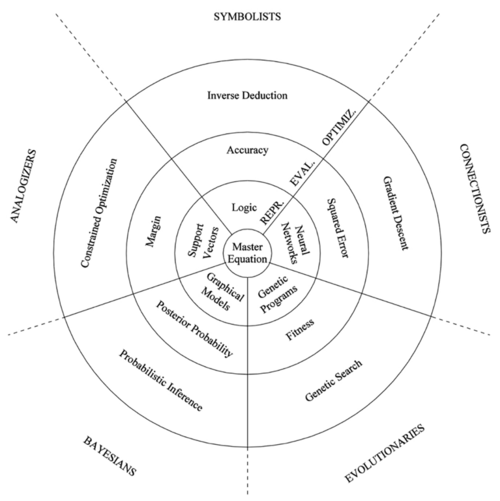
\includegraphics[scale=0.75]{ml-tribes.png}
  \caption{Machine Learning Tribes}
  \label{fig:congress}
\end{figure}
The other more mainstream approach of classification comes from machine learning community. 
\begin{figure}[H]
\centering
  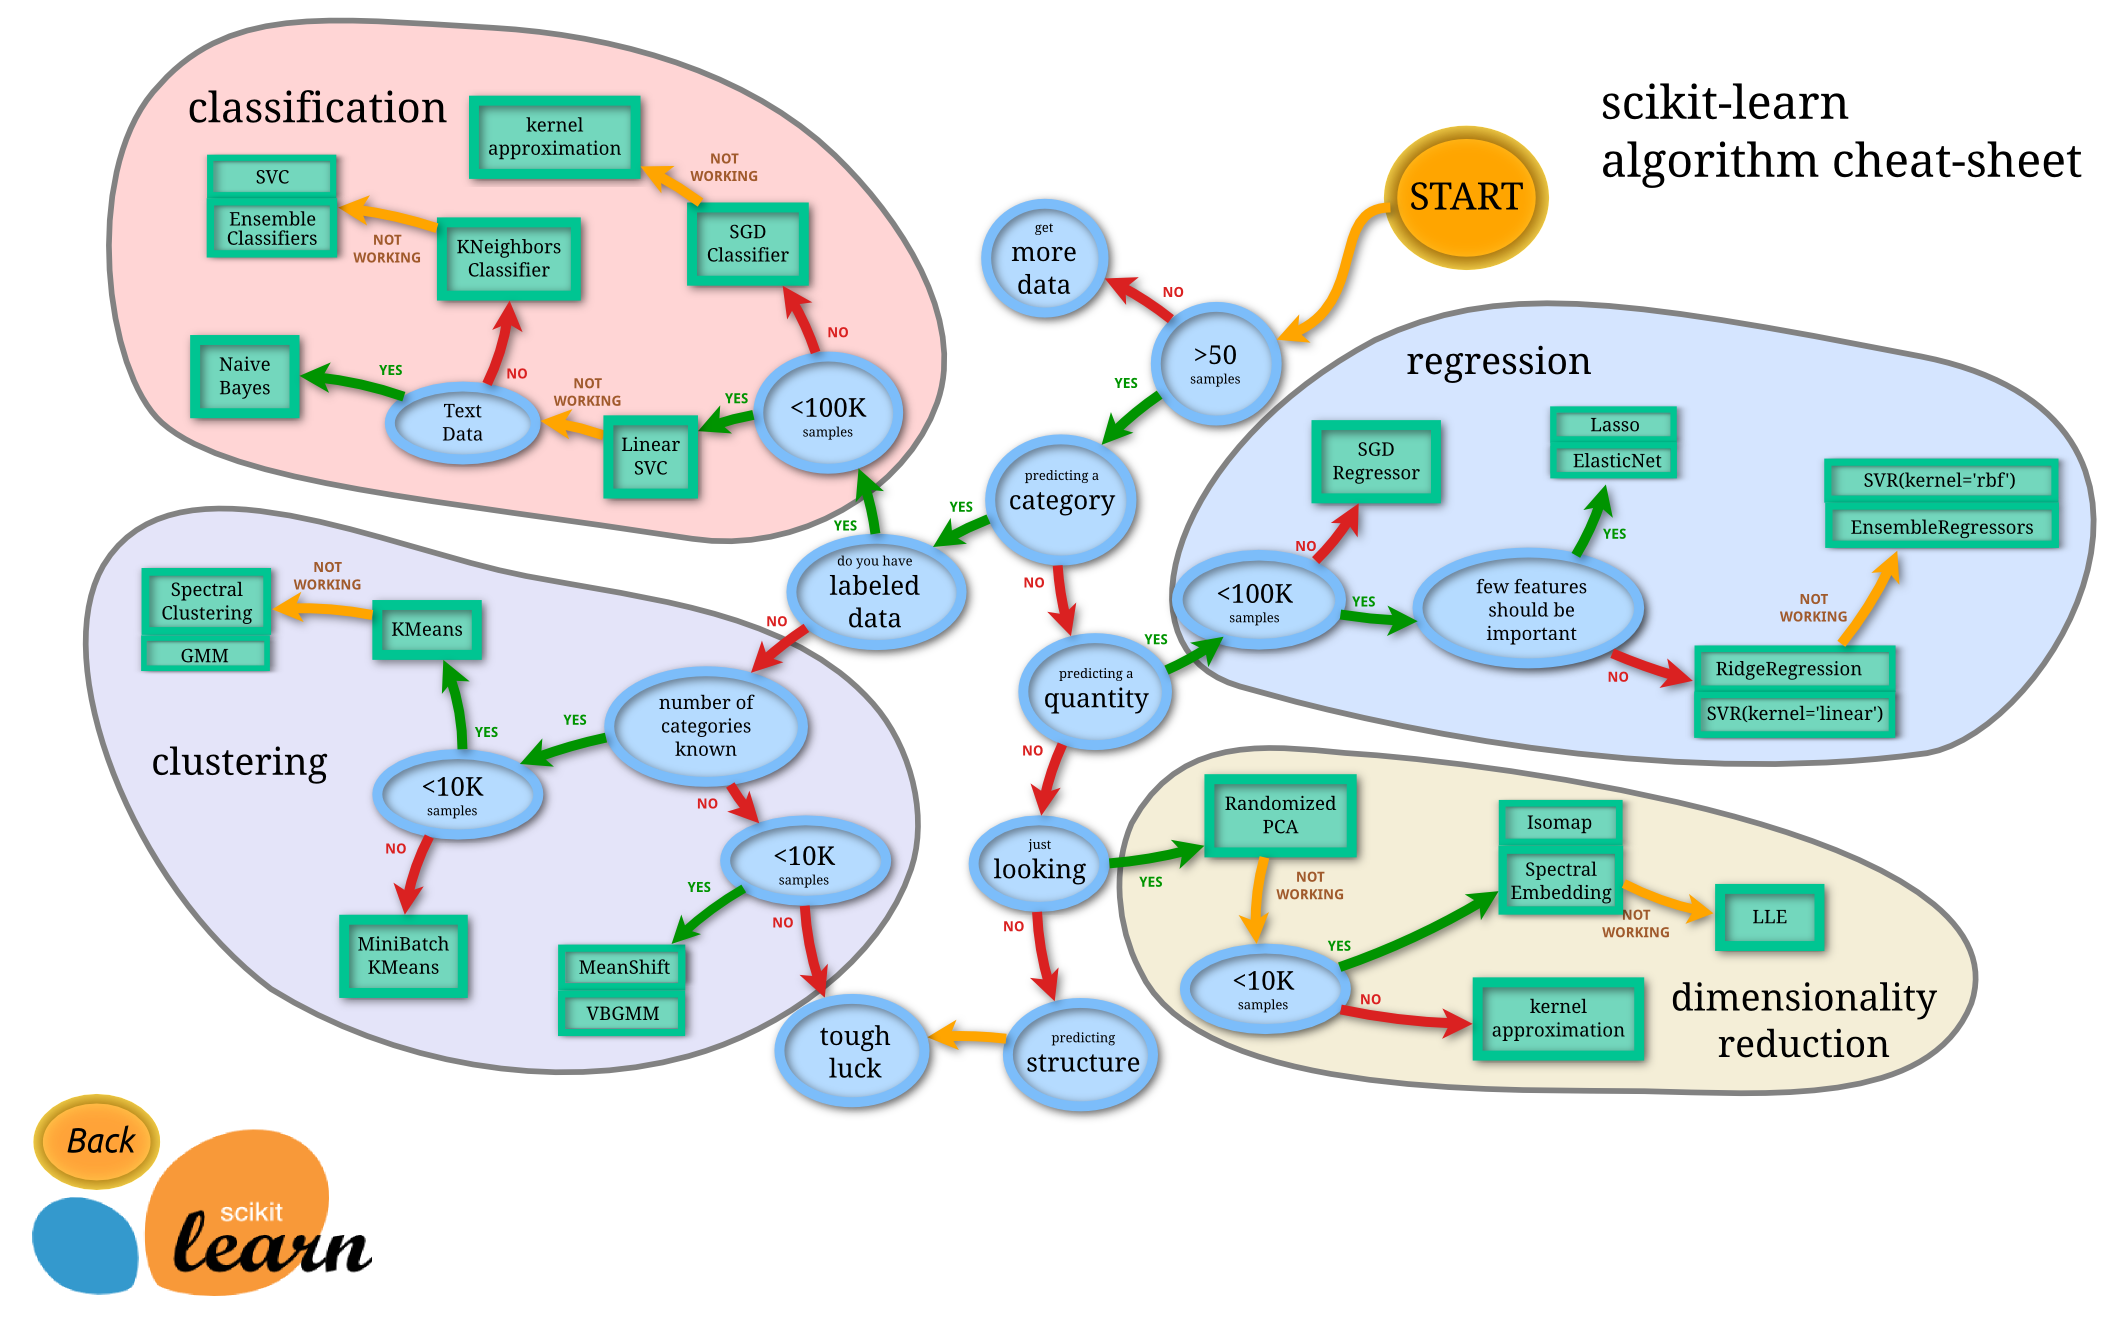
\includegraphics[width=\linewidth]{ml-map.png}
  \caption{Machine Learning Library Techniques}
  \label{fig:congress}
\end{figure}

Statistics uses probability theory to model distributions from which samples are typically drawn to use inductive inference for understanding any phenomenon. The new discipline of machine learning broadly has two kinds of learning techniques based on (i) parameters of distributions and (ii) distribution free models  based on samples for out-of-sample prediction of independent variables of interest. The core statistical distributions are very clearly explained on the blog of cloudera http://blog.cloudera.com/blog/2015/12/common-probability-distributions-the-data-scientists-crib-sheet/. 

\begin{figure}[H]
\centering
  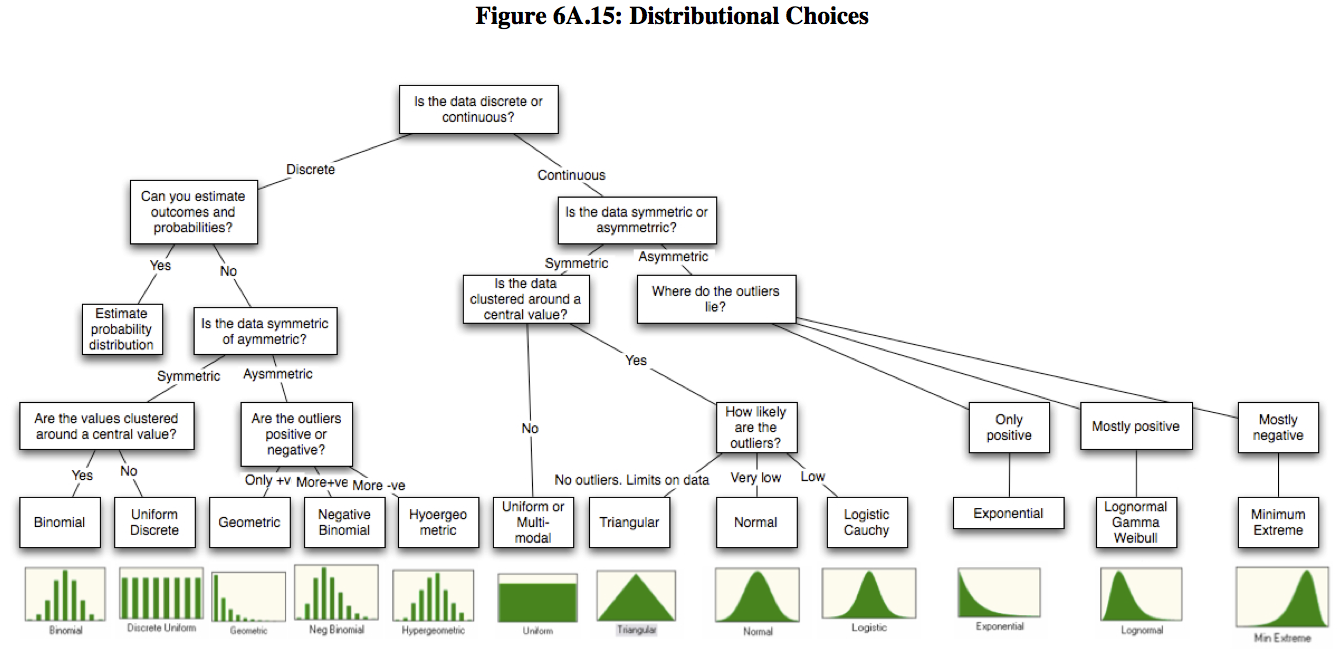
\includegraphics[width=\linewidth]{distributions.png}
  \caption{Statistical Distributions}
  \label{fig:congress}
\end{figure}

\section{Complexity P=NP, UGC}
Beautiful area of computational complexity in the context of the boundary between easy and hard optimization problems. Awesome talk on youtube by Eric DeMaine of MIT explains the basics. I also read a survey paper titled Computational Complexity for Physicists by Stephan Mertens that provides an excellent survey of topic. One of the remarkable things I read recently that had drawn my attention is from the latest volume of Fundamental Algorithms by the great Donald Knuth. He passingly mentions his belief of the complexity class \textit{P being equal to NP and our inability to not prove it}. This is pretty significant coming from someone like him when the majority of the leading researchers feel otherwise. 

\begin{figure}[H]
\centering
  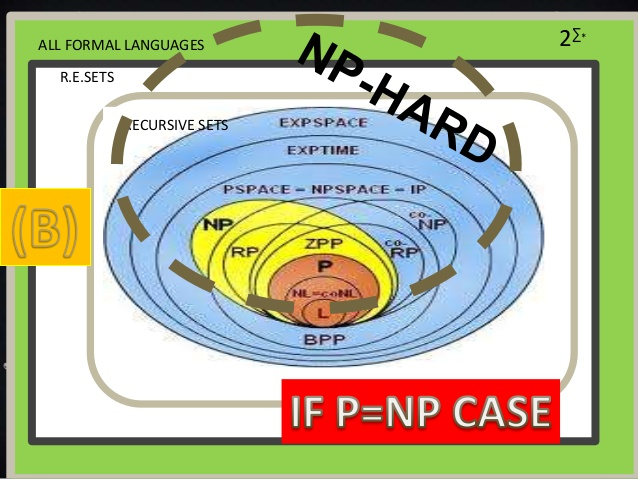
\includegraphics[scale=0.5]{complexity.jpg}
  \caption{Computational Complexity Classes}
  \label{fig:congress}
\end{figure}

\section{Application Areas of Knowledge}
\subsection{Economics and Finance}
All economic and financial activities require multiple entities and interaction between them. A natural view of this in terms of some kind of graph. The fundamental traditional model to understand any such activity uses the following. 
\begin{figure}[H]
\centering
  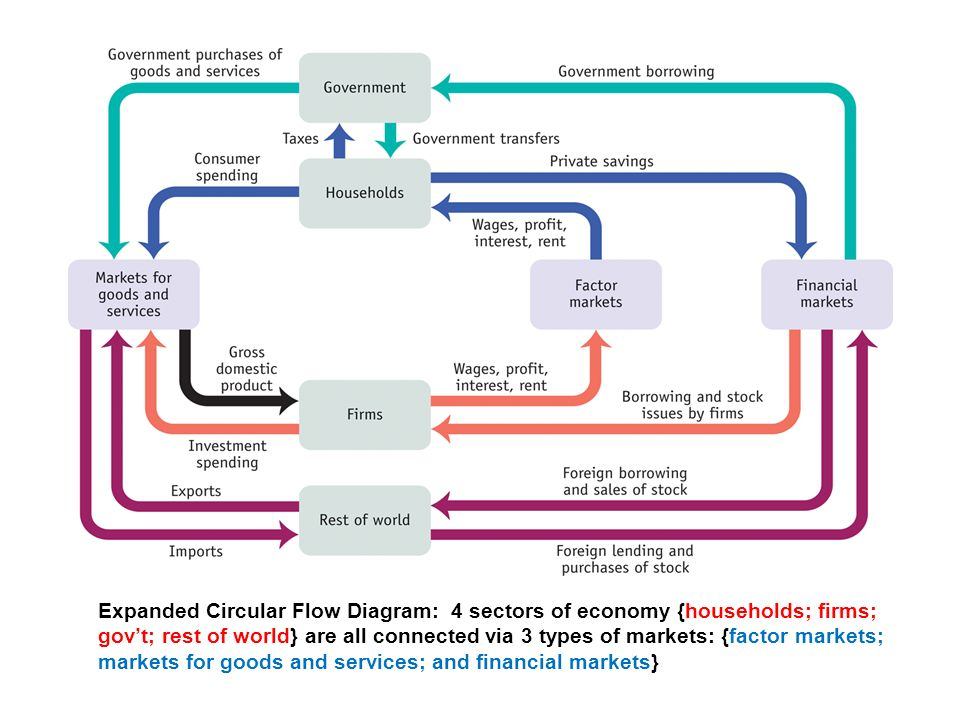
\includegraphics[scale=0.65]{economy.jpg}
  \caption{Economy Graph}
  \label{fig:congress}
\end{figure}

\subsection {Domain : Structure of civics}
Both USA and India have a similar political structure at a very high level with three branches of government, namely, legislative, judicial and executive. They also share two major sections of parliament/congress of Lok Sabha/House of Represetatives and Rajya Sabha-Senate with similar kind of appointment durations. However, the US Senate seems more powerful than Rajya Sabha. West Bengal has 44 MPs , i.e., representatives in the Lok Sabha and lot more MLAs. On the other hand, there are 2 house representives from Georgia, both Republicans although the local state district representative of Lawrenceville is a Democrat, Mr Park. 
\begin{figure}[H]
\centering
  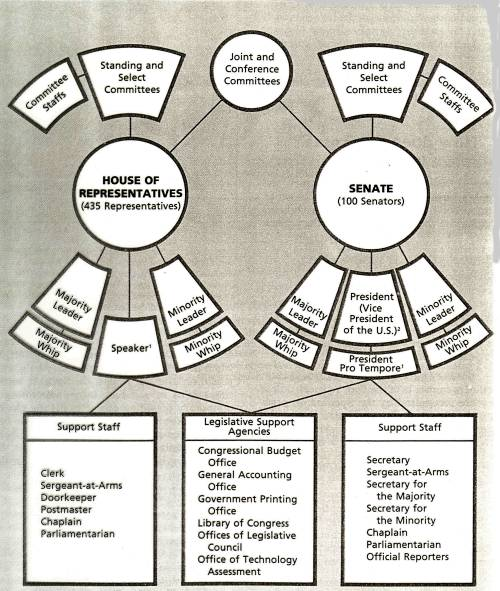
\includegraphics[scale=0.65]{congress.jpg}
  \caption{Congress structure}
  \label{fig:congress}
\end{figure}


\subsection{Life : Biology, Genetics etc.}
\subsection{Transportation : Automobiles}
\subsection{Energy : }

\end{document}  